\documentclass{beamer}
\usepackage[utf8]{inputenc}
\usepackage[T1]{fontenc}
\usepackage[english]{babel}
\usepackage{graphicx}
\usepackage{times}
\usepackage{caption}
\captionsetup{labelformat=empty,labelsep=none}

\usetheme{AGH}

\title[Praca magisterska]{Opracowanie systemu inwestycyjnego opartego na wybranych japońskich \\technikach analizy wykresów}

\author[T. Górny]{Tomasz Górny}

\date[2012]{15.10.2012}

\institute[AGH]
{Wydział EAIiE\\ 
Katedra Informatyki Stosowanej\\
promotor: dr inż. Mirosław Gajer
}

\setbeamertemplate{itemize item}{$\maltese$}

\begin{document}

{
%\usebackgroundtemplate{
\includegraphics[width=\paperwidth]{titlepage}} % wersja angielska
\usebackgroundtemplate{
\includegraphics[width=\paperwidth]{titlepagepl}} % wersja polska
 \begin{frame}
   \titlepage
 \end{frame}
}

%---------------------------------------------------------------------------

\begin{frame}
\frametitle{Cele}

\begin{itemize}

\item Porównanie internetowych platform handlowych
\item Stworzenie automatycznej strategii inwestycyjnej
\item Zweryfikowanie sprawdzalności świec japońskich

\end{itemize}

\end{frame}

%---------------------------------------------------------------------------


\begin{frame}
\frametitle{Założenia}

\begin{itemize}

\item wykorzystanie platformy MetaTrader
\item język MQL4
\item analiza rynku FOREX
\item testowanie EUR-USD

\end{itemize}

\end{frame}

%---------------------------------------------------------------------------

\begin{frame}
\frametitle{Główne funkcje}

\begin{itemize}

\item Analiza danych w czasie rzeczywistym
\item Rozpoznawanie głównych formacji 
\item Możliwość optymalizacji strategii
\item Automatyczne przeprowadzanie transakcji
\item Uniwersalność

\end{itemize}

\end{frame}

%---------------------------------------------------------------------------

\begin{frame}
\frametitle{Budowa świecy japońskiej}
\begin{figure}[ht]
\begin{center}
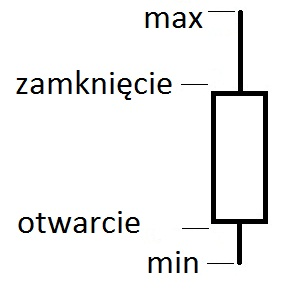
\includegraphics[width=5cm]{candle.jpg}
\caption{Budowa świecy japońskiej}
\end{center}
\end{figure} 


\end{frame}

%---------------------------------------------------------------------------

\begin{frame}
\frametitle{Formacja młot}
\begin{figure}[ht]
\begin{center}
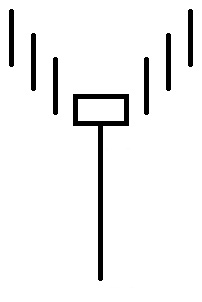
\includegraphics[width=4cm]{hammer.jpg}
\caption{Budowa formacji młot}
\end{center}
\end{figure} 


\end{frame}

%---------------------------------------------------------------------------

\begin{frame}
\frametitle{Formacja gwiazda wieczorna}
\begin{figure}[ht]
\begin{center}
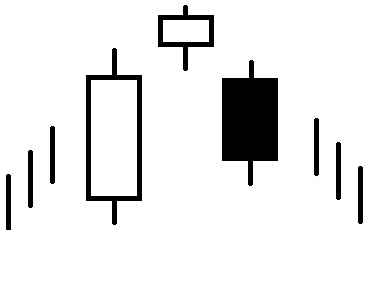
\includegraphics[width=6cm]{star.jpg}
\caption{Budowa formacji gwiazda wieczorna}
\end{center}
\end{figure} 


\end{frame}

%---------------------------------------------------------------------------

\begin{frame}
\frametitle{Optymalizacja}
\begin{figure}[ht]
\begin{center}
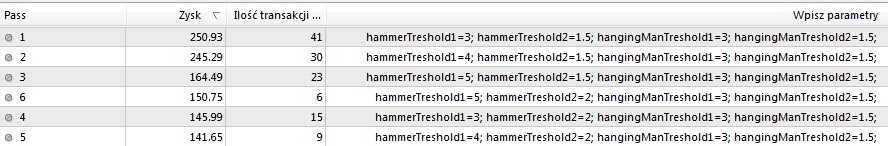
\includegraphics[width=12cm]{result.jpg}
\caption{Wyniki przykładowej optymalizacjij}
\end{center}
\end{figure} 


\end{frame}

%---------------------------------------------------------------------------

\begin{frame}
\frametitle{Algorytm}
\begin{figure}[ht]
\begin{center}
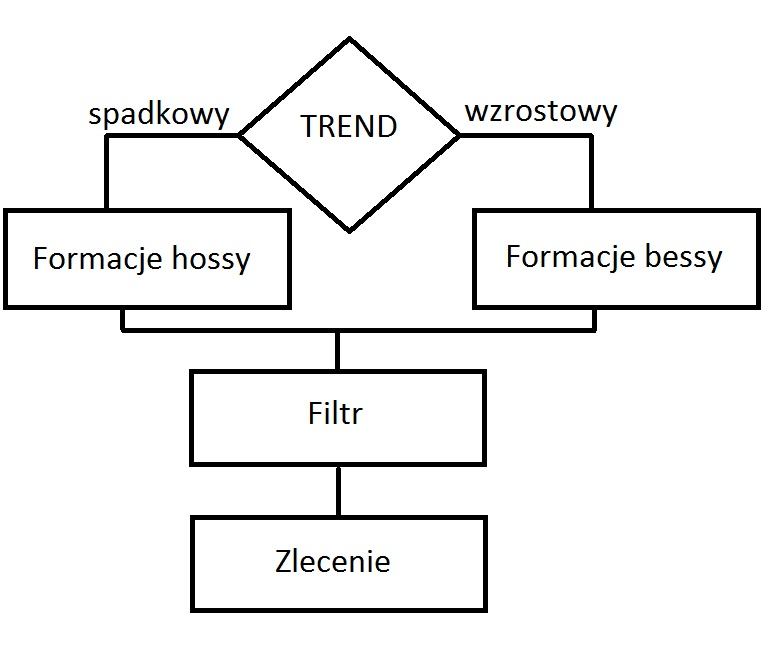
\includegraphics[width=7cm]{algorytm.jpg}
\caption{Schemat algorytmu}
\end{center}
\end{figure} 


\end{frame}

%---------------------------------------------------------------------------

\begin{frame}
\frametitle{Przykład}
\begin{figure}[ht]
\begin{center}
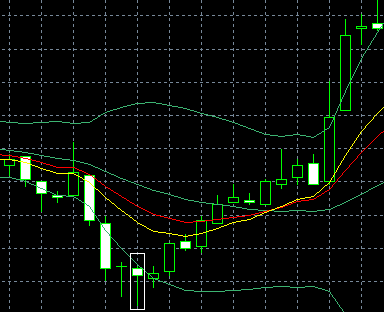
\includegraphics[width=7cm]{sample.png}
\caption{Sposób działania algorytmu}
\end{center}
\end{figure} 


\end{frame}

%---------------------------------------------------------------------------

\begin{frame}
\frametitle{Koniec}
\begin{center}
Dziękuję za uwagę
\end{center}

\end{frame}

%---------------------------------------------------------------------------


\end{document}

